

\section{Experimental setup}
\label{sec:experiment}
\label{sec:experiment}

The analysis is carried out with data samples of pp collisions at $\sqrt{s} = 13$~TeV collected from 2016 to 2018 during the LHC Run 2 period. The full description of the ALICE detector and its performance in the LHC Run 2 can be found in~\cite{Aamodt:2008zz,Abelev:2014ffa}. The present analysis utilizes the V0~\cite{Abbas:2013taa}, the Inner Tracking System (ITS)~\cite{aliceITS}, and the Time Projection Chamber (TPC)~\cite{aliceTPC} detectors.

The V0 detector consists of two stations placed on both sides of the interaction point, V0A and V0C, each made of 32 plastic scintillator tiles, covering the full azimuthal angle within the pseudorapidity intervals $2.8 < \eta < 5.1$ and $-3.7 < \eta < -1.7$, respectively. The V0 is used to provide a minimum bias (MB) and a high-multiplicity (HM) trigger. The minimum bias trigger is obtained by a time coincidence of V0A and V0C signals. The charged particle multiplicity selection is done on the sum of the V0A and V0C signals, which is denoted as V0M. The high-multiplicity trigger requires that the V0M signal exceeds 5 times the mean value measured in minimum bias collisions, selecting the 0.1\% of MB events that have the largest V0 multiplicity. The analyzed data samples of minimum bias and high-multiplicity pp events at $\sqrt{s}=$~13 TeV correspond to integrated luminosities of 19 nb$^{-1}$ and 11 pb$^{-1}$, respectively~\cite{ALICE-PUBLIC-2016-002}.

The primary vertex position is reconstructed from the measured signals in the Silicon Pixel Detector (SPD), which forms the innermost two layers of the ITS. Reconstructed primary vertices of selected events are required to be located within 8~cm from the center of the detector along the beam direction. The probability of pileup events is about 0.6\% in MB events. Pileup events can be resolved and are rejected if the longitudinal displacement of their primary vertices is larger than 0.8 cm.

Charged-particle tracks are reconstructed by the ITS and TPC, which are operated in a uniform solenoidal magnetic field of 0.5~T along the beam direction. The ITS is a silicon tracker with six layers of silicon sensors where the SPD~\cite{Santoro2009:ALICESPD} comprises the two innermost layers, the next two layers called the Silicon Drift Detector (SDD), and the outermost layers named the Silicon Strip Detector (SSD). The ITS and TPC, covering the full azimuthal range, have acceptances up to $|\eta| < 1.4$ and 0.9, respectively, for detection of charged particles emitted within 8 cm from the primary vertex position ($z_\mathrm{vtx}$) along the beam direction. The tracking of charged particles is done with the combined information of the ITS and TPC that enables the reconstruction of tracks down to 0.15~GeV/$c$, where the efficiency is about 65\%. The efficiency reaches 80\% for intermediate $\pt$, 1 to 5~GeV/$c$. The $\pt$ resolution is around 1\% for primary tracks with $\pt<$~1~GeV/$c$, and linearly increases up to 6\% at $\pt \sim$ 40~GeV/$c$~\cite{Contin_2012:ITSPTRES}.
%https://arxiv.org/pdf/1910.14400.pdf %https://arxiv.org/abs/1402.4476

The charged particle selection criteria are optimized to make the efficiency uniform over the full TPC volume to mitigate the effect of small regions where some of the ITS layers are inactive. The selection consists of two track classes. Those belonging to the first class are required to have at least one hit in the SPD. Tracks from the second class do not have any SPD associated hit and their initial point is instead constrained to the primary vertex~\cite{Adam:2015ewa}.

\section{Analysis procedure}
\label{sec:ana}
\subsection{Two-particle angular correlations}
Two-particle angular correlations are measured as a function of the relative azimuthal angle ($\Delta\varphi$) and the relative pseudorapidity ($\Delta\eta$) between a trigger and associated particle,
\begin{eqnarray}
\frac{1}{N_{\rm{trig}}} \frac{ \rm{d}\it{}^{2} N_{\rm{pair}} }{ \rm{d} \Delta\eta \rm{d}\Delta\varphi} = B(0, 0)\frac{S(\Delta\eta, \Delta\varphi)}{B(\Delta\eta, \Delta\varphi)}  \Big\lvert_{\pttrig,\,\ptassoc}\quad , 
\label{eq:corrfunction}
\end{eqnarray}
where the trigger and associated particles are defined from different transverse momenta ($p_\mathrm{T}$) ranges. $N_{trig}$ and $N_{pair}$ are the number of trigger particles and trigger-associated particle pairs respectively. $S(\Delta\eta, \Delta\varphi)$ corresponds to the average number of pairs in the same event and $B(\Delta\eta, \Delta\varphi)$ to the number of pairs in mixed events. $B (0,0)$ represents the normalization of $B(\Delta\eta, \Delta\varphi)$, and by dividing $S(\Delta\eta, \Delta\varphi)$ with $B(\Delta\eta, \Delta\varphi)/B (0,0)$ the acceptance effects are corrected for. The track reconstruction efficiency is corrected for on the right-hand side of Eq.~\ref{eq:corrfunction}. This analysis is done for multiple centrality classes ($0-0.1\%$, $1-5\%$, $5-20\%$ and $20-60\%$), and for each multiplicity class, the pairs in mixed events are required to have primary vertices within the same 2 cm wide $z_{vtx}$ interval~\cite{KOPYLOV1974472:evtmixing,Adam:2016tsv}. As a last step, the correlation functions are averaged over the vertex bins which results in the final per-trigger yield.

%Explain ridge yields

From the final per-trigger yield, ridge yields are extracted for different multiplicity classes and $\pt$ intervals at large $\Delta\eta$. The selection of the large $\Delta\eta$ range is based on where the tracking quality -- efficiency and precision -- is the best, which is at $1.6<|\Delta\eta|<1.8$. The reported $\pt$ cut is at $\pt>$~1~GeV/$c$ since at lower $\pt$, the jet-like contribution extends into the $\Delta\eta$ range that is measured. In this region, the per-trigger yield, $\Delta\varphi$, is expressed as
\begin{eqnarray}
\frac{1}{N_{\rm{trig}}} \frac{ \rm{d}\it{}N_{\rm{pair}} }{ \rm{d}\Delta\varphi } = \int_{1.6<|\Delta \eta|<1.8} \left( \frac{1}{\it{N}_{\rm{trig}}} \frac{ \rm{d}\it{}^{2} N_{\rm{pair}} }{ \rm{d}\Delta\eta d\Delta\varphi} \right) \dfrac{1}{\delta_{\Delta\eta}} \rm{d}\Delta \eta - C_{\rm{ZYAM}}\quad ,
\end{eqnarray}
where $\delta_{\Delta\eta}=$~0.4 is the normalization factor to get the per-trigger yield per unit of pseudorapidity. The Zero-Yield-At-Minimum (ZYAM) procedure~\cite{Ajitanand:2005jj} is the method used to subtract the baseline of the correlation. 


\subsection{Extraction of flow via the Low-Multiplicity Template Fit Method}
Due to the strong jet fragmentation bias in small systems it has been difficult to fully understand the flow extraction methods in these systems, hence the low-multiplicity template fit have been used in order to remove the remaining non-flow contributions. %This method makes two assumptions; that $f_{\rm{LM}}(\Delta\varphi)$ only includes non-flow contributions, mainly from back-to-back jets correlations, and at the same time it does not include any flow modulations. 
It is assumed that there is no ridge in low-multiplicity events (60--100\%), i.e. that the away-side peak in these events, is mostly caused by jet fragmentations. Hence, by removing the measured correlation function in these events from measured correlation functions in high multiplicity events, no non-flow contributions are left in the correlation. This method is referred to as the low-multiplicity template fit, and is defined as
\begin{eqnarray}
f_{\rm{sig}}(\Delta\varphi) = G(1 + 2v_{2,2}\cos(2\Delta\varphi) + 2v_{3,3}\cos(3\Delta\varphi)) + Ff_{\rm{LM}}(\Delta\varphi)
\end{eqnarray}
where the $F$ parameter corresponds to the relative away-side jet-like contribution from the low-multiplicity ($60-100\%$) to the different high multiplicity classes. The $F$ parameter that is obtained from this fit is then used to scale the two-dimensional low-multiplicity correlation function templates before subtraction from the signal yield. 
After the removal, it is now possible to extract the flow modulations $v_{2,2}$ and $v_{3,3}$, again using the template fit defined as,
\begin{eqnarray}
\chi^{2} = \sum \dfrac{ ( f_{\mathrm{sig}}(\Delta\varphi) - ( G(1 + 2v_{2,2}\cos(2\Delta\varphi) + 2v_{3,3}\cos(3\Delta\varphi)) + Ff_{\mathrm{LM}}(\Delta\varphi) )^{2} }{ \sigma_{ f_{\mathrm{sig}}(\Delta\varphi)}^{2} +  (F\sigma_{ f_{\mathrm{LM}}(\Delta\varphi) ) })^{2} }
\end{eqnarray}

\begin{figure}[!t]
	\centering
	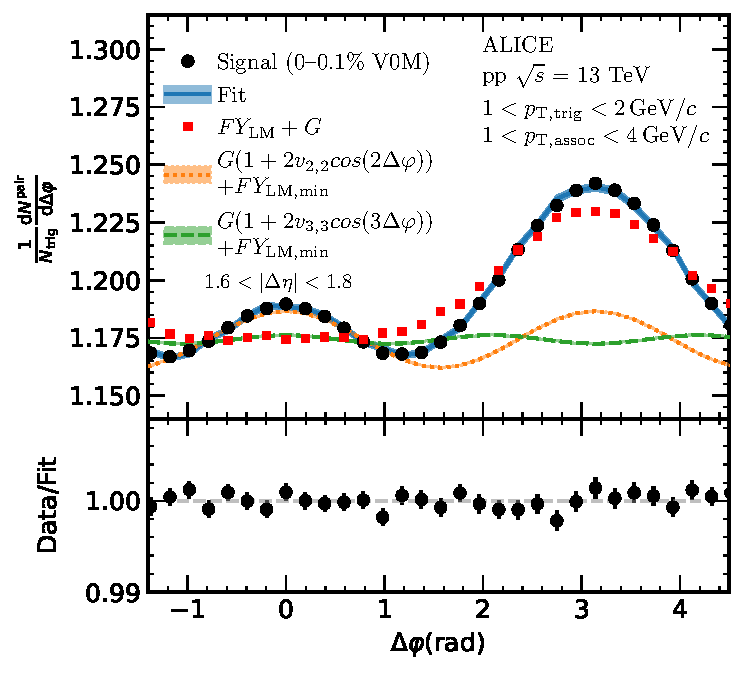
\includegraphics[width=0.8 \textwidth]{figures/Fig1_FlowExt.pdf} 
	\caption{The template fit results with the biased LM templates. The black markers shows the signal for the $0-0.1\%$ centrality class together with its fit shown as a blue band. The red squares correspond to the low multiplicity signal scaled with $F$. The orange and green curves correspond to the extracted $v_2$ and $v_3$ signals, respectively.}
	\label{fig:flowext}
\end{figure}

Figure~\ref{fig:flowext} shows the template fit results for pp collisions at 13 TeV and the $0-0.1\%$ centrality class events. The trigger particles are in the $p_\mathrm{T}$ range of $1<p_{\mathrm{T,trig}}<2$ GeV/c and the associated particles in $1<p_{\mathrm{T,trig}}<4$ GeV/c. The signal is shown together with its fit, and the ratio of the two giving a result around unity proves that the signal is successfully fitted. The scaled low-multiplicity yield that is subtracted from the signal is shown in red squares, and the extracted $v_2$ and $v_3$ as orange and green respectively. 
It is clear that after the removal, the away-side jet-fragmentation was successfully subtracted from the signal and that it was possible to extract $v_2$ and $v_3$. 

\begin{figure}[!th]
	\centering
	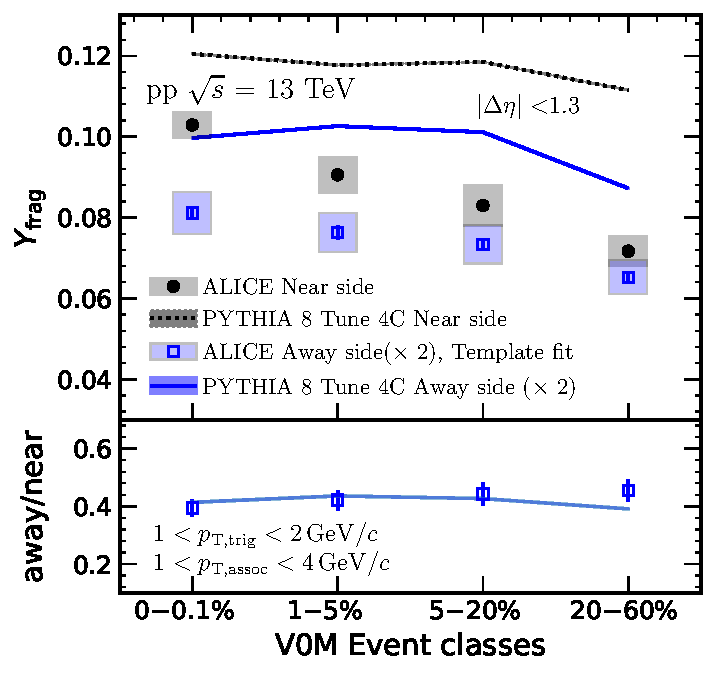
\includegraphics[width=0.8 \textwidth]{figures/Fig5_Plot_v2Mult.pdf} 
	\caption{$Y^{\rm{near}}$ and $Y^{\rm{away}}$ as a function of V0M multiplicity classes with both ALICE and PYTHIA data. The ratio includes the combined statistical and systematic errors in quadrature.}
	\label{fig:Ymult}
\end{figure}

The near-side jet-like yields are extracted from the near-side $\Delta\eta$ correlations, with the near-side $\Delta\eta$ correlations being defined at $|\Delta\varphi|<$~1.3 projected on the $\Delta\eta$ axis. The value 1.3 is chosen as the projection range in order to fully cover $\Delta\varphi_{\rm{min}}$. However, the away-side jet-like yield is measured indirectly as $Y^{\rm{away}} = Y^{\rm{away, LM}} \times F$, where $F$ is again the relative contribution of the away-side jet fragmentation yield between low- and high-multiplicity events. The $Y^{\rm{Away, LM}}$ is then directly measured by integrating the short-range $\Delta\varphi$ ($0<\Delta\varphi<\pi$) correlations with the assumption that there is no ridge in LM.
\begin{eqnarray}
Y^{\rm{frag}} = \int_{|\Delta \eta|<1.3} \left( \frac{1}{\it{N}_{\rm{trig}}} \frac{ \rm{d}\it{}N_{\rm{pair}} }{ \rm{d}\Delta\eta } \right) \rm{d} \Delta\eta \quad.
\end{eqnarray}

Figure~\ref{fig:Ymult} presents $Y^{\rm{near}}$ and $Y^{\rm{away}}$, for both ALICE and PYTHIA 8 Tune 4C generated data as a function of multiplicity in pp collisions at 13 TeV. The transverse momentum range for trigger particles is $1<p_\mathrm{T,trig}<2$ GeV/c and for associated particles $1<p_\mathrm{T,assoc}<4$ GeV/c. ALICE data points are shown as circle and square markers, whereas PYTHIA is shown as lines. The near-side yields are shown in black and the away-side yields in blue. The jet fragmentations are not reproduced by PYTHIA in either near- or away-side, and as a consequence, the $F$ parameter nicely estimates the relative away-side contribution from low-multiplicity events to high multiplicity events.

\subsection{Event scale selections}
As a continuation of the two particle correlations analysis with the template fit method, different event scale selections are investigated. By selecting events that includes a hard jet or a high-$\pt$ leading particle within the mid-rapidity region, it is possible to study the ridge yield further. This event scale is set by requiring a minimum $\pt$ of the leading track ($\ptlead$), i.e. track with the highest momentum in an event, or the reconstructed jet ($\ptjet$) at midrapidity. The leading particle track requires to be within $|\eta|<0.9$ and $0<\phi<2\pi$, and the jets are reconstructed with the anti-$k_{\rm{T}}$ algorithm~\cite{Cacciari:2008gp,Cacciari:2011ma}, with $R=$~0.4, for only charged particles. In this analysis the $\pt$ scheme is used as the recombination scheme. Just as the leading particle tracks, the jets are selected in the full azimuthal angle ($0<\phi<2\pi$) but in an $\eta$-range of $|\eta_\mathrm{jet}|<0.4$. The $\pt$ of jets $\ptjet$ is corrected for the underlying event density that is measured using the $k_{\rm{T}}$ algorithm with $R=$~0.2~\cite{Acharya:2018eat}.




%%%%%%%%%%%%%%%%%%%%%%%%%%%%%%%%%%%%%%%%%%%%%%%%%%%%%%%%%%

\section{Systematic uncertainties of the measured yields}
\label{sec:uncertainties}

The systematic uncertainties of $Y^{\rm{ridge}}$ and $Y^{\rm{near}}$ are estimated by varying the analysis selection criteria and corrections and are summarized in Tab.~\ref{tab:syst}.

\begin{table}[h!]
\caption{The relative systematic uncertainty of $Y^{\rm{ridge}}$ and $Y^{\rm{near}}$. Numbers given in ranges correspond to minimum and maximum uncertainties.}
\centering
\begin{tabular}{c|cc}
\hline 
\multirow{2}{*}{Sources}  & \multicolumn{2}{c}{Systematic uncertainty (\%)} \\\cline{2-3} 
         & $Y^{\rm{ridge}}$ & $Y^{\rm{near}}$ \\ \hline 
Pileup rejection    	& $\pm$0.8--3.9    &$\pm$0.2--2.2	\\ 
Primary vertex	        & $\pm$0.5--2.4	   &$\pm$1.1	\\ 
Tracking		        & $\pm$2.0--4.0    &$\pm$1.5--3.4	\\ 
ZYAM		        	& $\pm$2.1--5.1	   &$\pm$2.2--4.8	\\ 
Event mixing	    	& $\pm$1.0--4.4	   &$\pm$0.5--1.7	\\ 
Efficiency correction	& $\pm$2.5 	    &$\pm$3.1	\\  
Jet contamination   	& $-$18.8--25.9 ($\pt<$~2~GeV/$c$)	&N.A.	\\ \hline 
Total (in quadrature)			& $^{+\rm{4.9}\textrm{--}\rm{9.4}}_{-\rm{19.4}\textrm{--}\rm{21.0}}$ & $\pm$3.9--7.3 \\ 
\hline 
\end{tabular}
\label{tab:syst}
\end{table}

The systematic uncertainties are independent of the event-scale selection except for $D_{\rm{ZYAM}}$ (see below), as expected, since the multiplicity is weakly dependent on the event scale and the ALICE detector is optimized for much higher multiplicities (Pb--Pb collisions), this is in agreement with our expectations.

The uncertainty associated to the pileup rejection is estimated by measuring the changes of results with different rejection criteria from the default one. It is mainly estimated by varying the minimal number of track contributors required for reconstruction of pileup event vertices from 3 to 5. The estimated uncertainty of $Y^{\rm{ridge}}$ is 0.8-3.9\%. The corresponding uncertainty of $Y^{\rm{near}}$ is estimated to be 0.2--2.2\%.
 
Another source of systematic uncertainty is related to the selected range of the primary vertex. The accepted range is changed from $|z_\mathrm{vtx}|<$ 8 cm to $|z_\mathrm{vtx}|<$ 6 cm. The narrower primary vertex selection allows one to test acceptance effects on the measurement. The estimated uncertainty of $Y^{\rm{ridge}}$ is 0.5--2.4\%. The uncertainty for $Y^{\rm{near}}$ is estimated to be 1.1\%.

An additional source of systematic uncertainty is related to the track selection criteria. The corresponding uncertainty is estimated by employing other track selection criteria, denoted global tracks, which are optimized for particle identification. The selection criteria of the global tracks are almost identical to the hybrid tracks. Each global track is required to have at least one SPD hit. Due to inefficient parts of the SPD, the azimuthal distribution of global tracks is not uniform.
The uncertainties associated with the track selection are estimated to be 2.0--4.0\% and 1.5--3.4\% for $Y^{\rm{ridge}}$ and $Y^{\rm{near}}$, respectively.

The systematic uncertainty of $Y^{\rm{ridge}}$ resulting from the ZYAM procedure is estimated by varying the range of the fit, which is used to find the minimum, from $|\Delta\varphi|<\pi/$2 down to $|\Delta\varphi|<1.2$. The estimated uncertainty of $Y^{\rm{ridge}}$ is 2.1--5.1\%. The corresponding uncertainty on $Y^{\rm{near}}$ is estimated by varying the range from $|\Delta\eta|<$~1.6 to $|\Delta\eta|<$~1.5 and 1.7. The estimated uncertainty of $Y^{\rm{near}}$ is 2.2\% for the unbiased case and increases to 4.8\% for the largest event-scale selections. This is the only systematic uncertainty for which a significant dependence on the event scale is observed, reflecting a non-negligible dependence of the near-side magnitude and shape on the event-scale selection.

The source of systematic uncertainty is associated to the choice of the width of $z_{\rm vtx}$ bins that are used in the event mixing method. The default value of 2\,cm is changed to 1\,cm. The resulting uncertainty of $Y^{\rm{ridge}}$ is 1.0--4.4\%.
The uncertainty for $Y^{\rm{near}}$ is about 0.5--1.7\%. The uncertainty from the efficiency correction for charged particles is estimated by comparing correlation functions of true particles with correlation functions of reconstructed tracks with the efficiency correction in simulation. The estimated uncertainties are 2.5\% and 3.1\% for $Y^{\rm{ridge}}$ and $Y^{\rm{near}}$, respectively. 

In the limited $\eta$-acceptance of ALICE, the ridge structure is not flat in $\Delta\eta$ suggesting that jet-like correlations (non-flow) could contribute, implying that they would impact the ridge-yield extraction. We stress that the models used for comparisons also contain such a non-flow effect, but differences in jet-like correlations between data and MC models could influence the interpretation. To account for the related uncertainty, the variation of the yield with $\Delta\eta$ between 1.5 and 1.8, which should be an upper limit of the residual jet-like contamination, is used as a systematic uncertainty of the ridge yield. The estimated upper limit of the uncertainty is $-$25.9\% for the 1.0~$<\pt<$~1.5~GeV/$c$ range,  $-$18.8\% for the 1.5~$<\pt<$~2.0 GeV/$c$ range,  $-$18.9\% for the 1.0~$<\pt<$~2.0~GeV/$c$ range, and negligible for $\pt>$~2.0~GeV/$c$. This uncertainty is considered only for the measured ridge yields.




